\documentclass[10pt,a4paper]{article}
\usepackage[T1]{fontenc}
\usepackage{lmodern}
\usepackage[margin=20mm]{geometry}
\usepackage{amsmath,amssymb,booktabs,longtable,array}
\usepackage{xcolor,hyperref,pgfplots}
\pgfplotsset{compat=1.18}
\definecolor{ink}{RGB}{30,43,63}
\definecolor{accent}{RGB}{11,94,120}
\hypersetup{colorlinks=true,urlcolor=accent,linkcolor=accent}
\setlength{\parskip}{6pt}
\setlength{\parindent}{0pt}
\begin{document}
{\Large\bfseries\color{ink} A063 -- Hicks/Hill Euler Separatrix Falsifier}\par
{\large Scientific report -- v0.1.1}\par
\smallskip
\textbf{Scope:} Exact-field analytic reference, interface convergence, and numerically closed toroidal streamline candidate.\\
\textbf{Evidence:} Python/SciPy FP64, analytical/synthetic control only. \textbf{Not} canonical v1.0.7 native certification.\\
\textbf{Blind status:} no target particle labels, canonical masses or SST parameter fitting.
\vspace{2mm}\hrule
\section{Executive verdict}
A total of \textbf{10 PASS}, \textbf{3 UNRESOLVED}, and \textbf{0 FAIL} gates were recorded. The vortex-field reference is consistent with its prescribed accuracy gates; the original global topological/stability gate \texttt{H7}, the new trefoil/tube gate \texttt{H7B}, and independent native certification \texttt{H8} remain \texttt{UNRESOLVED}. A \texttt{PASS} of \texttt{H7A} only establishes a \emph{numerically closed T(3,4) streamline candidate}.

This report reads the additive v0.1.1 result JSONs. No older A063 v0.1.0 verdict is changed or migrated. Calculations are dimensionless with representative sphere radius $a=1$, density $\rho=1$ and predefined amplitude $A=1$.

\section{Exact Euler controls}
For cylindrical coordinates $(s,\phi,z)$ and the sphere $r^2=s^2+z^2\leq a^2$, the streamfunction and velocity in a sphere-comoving frame are
\begin{align}
J(x)&=\frac{\sin x}{x}-\cos x,\\
\psi_\lambda(r,\theta)&=A\left[J(\lambda r/a)-\frac{r^2}{a^2}J(\lambda)\right]\sin^2\theta,\\
(u_s,u_\phi,u_z)&=\left(-\frac{\psi_z}{s},\frac{\lambda\psi}{as},\frac{\psi_s}{s}\right).
\end{align}
At $\lambda=0$ a separate cancellation-safe Hill limiting field is used. The special families satisfy
\begin{align}
J(\lambda_1)=0\quad &(\text{Beltrami family}),\\
3J(\lambda_2)-\lambda_2\sin\lambda_2=0\quad &(\text{zero-translation family}).
\end{align}
With the local velocity gradient and Euler pressure obtained from the same analytic field, the interior reference checks
\begin{equation}
\nabla\cdot\mathbf u=0,\qquad (\mathbf u\cdot\nabla)\mathbf u+\frac{\nabla p}{\rho}=0,
\qquad \nabla\times\mathbf u=\frac{\lambda_1}{a}\mathbf u\ \text{for the Beltrami solution}.
\end{equation}

\textbf{Methodological correction from v0.1.0:} the residual maxima are now computed \emph{separately} for Hill, first Beltrami, and first zero-translation Hicks; the former H3 pooled Euler/divergence maxima from distinct families. Four finite-difference steps, $h/a\in\{4,2,1,0.5\}\times10^{-4}$, are compared for each family.

\begin{center}\small
\begin{tabular}{lrr}
\toprule
Reference & Max Euler residual (finest) & Max $|\nabla\cdot\mathbf u|$ (finest)\\
\midrule
Hill & 9.22e-09 & 4.36e-12\\
Beltrami & 8.87e-07 & 3.26e-08\\
Zero translation & 4.26e-06 & 1.08e-07\\
\bottomrule
\end{tabular}
\end{center}
The finest relative Euler error reduction ratios (previous step / finest step) exceed 2.5 for all three cases. These are finite-sample diagnostics, not global validated error bounds.

\section{Full-latitude material boundary and continuity}
The spherical separatrix is tested at 121 polar angles in each of three fields. The analytic no-flux condition $\mathbf u\cdot\mathbf n=0$ is evaluated on the sphere. Interior/exterior jumps in tangential velocity and pressure are measured at $r=a(1\pm\epsilon)$ for $\epsilon\in\{10^{-3},10^{-4},10^{-5}\}$.

\begin{center}\small
\begin{tabular}{lrrr}
\toprule
Field & $\Delta u(10^{-3})$ & $\Delta u(10^{-5})$ & $\Delta p(10^{-5})$\\
\midrule
Hill & 0.005988 & 5.995e-05 & 4.5e-05 \\
Hicks\_Beltrami\_1 & 0.02157 & 0.0002157 & 0.0003848 \\
Hicks\_static\_1 & 0.03169 & 0.0003169 & 3.425e-13 \\
\bottomrule
\end{tabular}
\end{center}
The jumps decay with radial offset for all fields. The latitude scan excludes only small caps $\theta<0.06$ and $\pi-\theta<0.06$, which remain outside this finite-sample claim. A smooth-interface test does not prove dynamical self-confinement.

\section{First rational-winding torus-line test}
On the first Beltrami family we integrate the Poincar\'e return map of the meridional plane and define
\begin{equation}
W(s_0)=\frac{\Delta\phi}{2\pi}\quad\text{per complete meridional circulation}.
\end{equation}
The target $W=3/4$ is bracketed by two independent sampled curves, then solved using Brent's method. Continuous three-dimensional integration over four meridional periods independently tests closing at a primitive $(p,q)=(3,4)$ winding:
\begin{align}
s_0/a&=0.968309830174,\\
W(s_0)&=0.750000000000,\\
(N_{\rm azimuth},N_{\rm meridional})&=(3.000000000,-4.000000000),\\
\|\mathbf x(4T)-\mathbf x(0)\|/a&=9.1832e-10.
\end{align}
\begin{center}
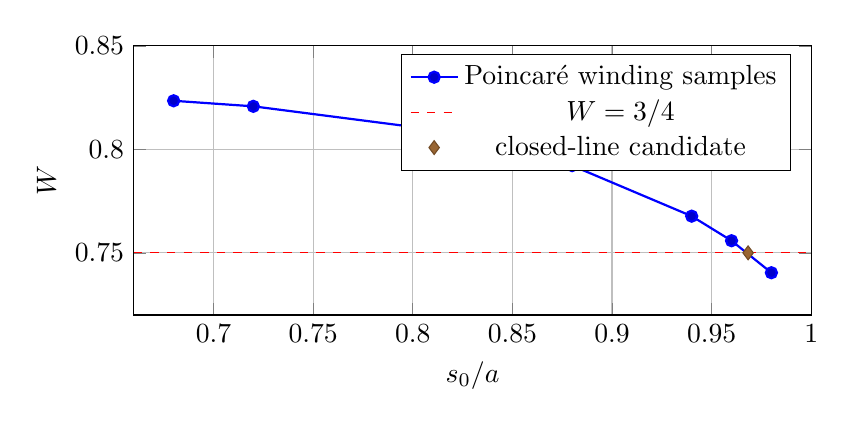
\begin{tikzpicture}
\begin{axis}[width=.84\textwidth,height=5cm,xlabel={$s_0/a$},ylabel={$W$},grid=major,legend pos=north east,xmin=.66,xmax=1,ymin=.72,ymax=.85]
\addplot+[mark=*,thick] coordinates {(0.68,0.8234505492) (0.72,0.82077351) (0.8,0.8108426301) (0.88,0.7921457722) (0.94,0.7677292566) (0.96,0.7558589923) (0.98,0.7404049981)};
\addlegendentry{Poincar\'e winding samples}
\addplot+[dashed,mark=none,domain=.66:1,samples=2] {0.75};
\addlegendentry{$W=3/4$}
\addplot+[only marks,mark=diamond*,mark size=2.5pt] coordinates {(0.968309830174,0.75)};
\addlegendentry{closed-line candidate}
\end{axis}
\end{tikzpicture}
\end{center}
\textbf{Allowed claim:} a numerical $T(3,4)$ \emph{streamline candidate} on an axisymmetric invariant torus, with monotone meridional phase and positive minimum radius. This does \textbf{not} independently certify a knot isotopy (e.g., with an Alexander polynomial), and does not show a finite-radius vortex \emph{tube}, an electron, or nonlinear Euler stability. It also does not globally exclude trefoil $T(2,3)$ from higher modes or other parameter ranges.

\section{Analytic bridges for the existing SST falsifiers}
\textbf{A046 pressure--vorticity:} tests $\nabla^2p=-\rho\,\partial_i u_j\partial_j u_i$ in the incompressible Euler field, without interpreting $p$ as gravitation. Maximum sampled pressure--Poisson absolute residual: $0.00028$.

\textbf{A057 finite-volume reference:} computes total laboratory-frame kinetic energy from interior volume quadrature plus the exact exterior dipole energy. Uniform far-field kinetic energy is not integrated in the translating frame. No constant-circulation normalization or physical mass-ratio inference is performed.
\begin{center}\small
\begin{tabular}{lrrr}
\toprule
Field & Interior $E$ & Exterior $E$ & Total $E$\\
\midrule
Hill & 3.440792 & 1.047198 & 4.48799 \\
Beltrami\_1 & 98.49107 & 8.953734 & 107.4448 \\
Static\_1 & 152.0015 & 3.671525e-31 & 152.0015 \\
\bottomrule
\end{tabular}
\end{center}

\section{Gate ledger and remaining qualifications}
\small
\begin{longtable}{@{}p{12mm}p{24mm}p{112mm}@{}}
\toprule
Gate & Status & Registered question\\\midrule\endhead
\texttt{H0} & \texttt{PASS} & Versioned source/protocol bytes match release seal? \\
\texttt{H1} & \texttt{PASS} & Do analytical roots satisfy registered equations? \\
\texttt{H2} & \texttt{PASS} & Does Hill zero-swirl control converge under finite-difference refinement? \\
\texttt{H3} & \texttt{PASS} & Does first Hicks Beltrami field satisfy curl(u)=k*u, Euler and divergence under refinement? \\
\texttt{H4} & \texttt{PASS} & Does lambda2 first Hicks mode have zero translation and a convergent stationary Euler field? \\
\texttt{H5} & \texttt{PASS} & Is the spherical boundary a material surface in all three exact fields? \\
\texttt{H6} & \texttt{PASS} & Do full-latitude interior/exterior pressure and velocity jumps converge to zero? \\
\texttt{H7} & \texttt{UNRESOLVED} & Are torus-knot accessibility and finite-core vortex-tube stability both certified? \\
\texttt{H7A} & \texttt{PASS} & Can a first-Beltrami streamline realize a closed rational 3/4 torus-winding candidate? \\
\texttt{H7B} & \texttt{UNRESOLVED} & Is trefoil T(2,3) accessible as a finite-core stable tube? \\
\texttt{H8} & \texttt{UNRESOLVED} & Has independent C++ FP64 certification run through v1.0.7 frozen protocol? \\
\texttt{H9} & \texttt{PASS} & Does exact pressure satisfy incompressible pressure-Poisson closure? \\
\texttt{H10} & \texttt{PASS} & Does finite laboratory-frame kinetic-energy quadrature converge? \\
\bottomrule
\end{longtable}
\normalsize
\textbf{Immediate next work:} independent topological invariant from sampled closed curve; global interval winding accessibility bounds for the trefoil; perturbed finite-core Euler-vortex-tube evolution and convergence; separate C++ FP64 native lane with the unmodified v1.0.7 instance protocol if certification is requested. No legacy falsifier framework migrations are necessary to render PDF reports.

\section*{Source and provenance}
Primary analytic source: W. M. Hicks (1899), \emph{Researches in Vortex Motion. Part III: On Spiral or Gyrostatic Vortex Aggregates}, \emph{Phil. Trans. R. Soc. A} \textbf{192}, 33--99, DOI: \href{https://doi.org/10.1098/rsta.1899.0002}{10.1098/rsta.1899.0002}. Classic reference: M. J. M. Hill (1894), \emph{On a Spherical Vortex}, \emph{Phil. Trans. R. Soc. A} \textbf{185}, 213--245, DOI: \href{https://doi.org/10.1098/rsta.1894.0006}{10.1098/rsta.1894.0006}. This release is an analytical Python control campaign, with no independent observational support for SST particle physics.\\
\footnotesize Run protocol SHA-256: \texttt{838a73226435889fe3cfee63053ee12d6a4a06d7cde67bb74a7ad02296038b99}.\\
Ledger SHA-256: \texttt{5283d44e0cf4a1ae4f514c6477169fac5e4be50e191daa5a637b07b9850740c4}.\\
Run timestamp (UTC): 2026-10-13T14:41:39.972373+00:00.
\end{document}
